\documentclass[a4paper,11pt]{article}
\usepackage{amsmath,amsthm,amsfonts,amssymb,amscd,amstext,vmargin,graphics,graphicx,tabularx,multicol} \usepackage[french]{babel}
\usepackage[utf8]{inputenc}  
\usepackage[T1]{fontenc} 
\usepackage[T1]{fontenc}
\usepackage{amsmath,amssymb}
\usepackage{pstricks-add,tikz,tkz-tab,variations}
\usepackage[autolanguage,np]{numprint} 
\usepackage{color}
\usepackage{ulem}

\setmarginsrb{1.5cm}{0.5cm}{1cm}{0.5cm}{0cm}{0cm}{0cm}{0cm} %Gauche, haut, droite, haut
\newcounter{numexo}
\newcommand{\exo}[1]{\stepcounter{numexo}\noindent{\bf Exercice~\thenumexo} : \marginpar{\hfill /#1}}
\reversemarginpar


\newcounter{enumtabi}
\newcounter{enumtaba}
\newcommand{\q}{\stepcounter{enumtabi} \theenumtabi.  }
\newcommand{\qa}{\stepcounter{enumtaba} (\alph{enumtaba}) }
\newcommand{\initq}{\setcounter{enumtabi}{0}}
\newcommand{\initqa}{\setcounter{enumtaba}{0}}

\newcommand{\be}{\begin{enumerate}}
\newcommand{\ee}{\end{enumerate}}
\newcommand{\bi}{\begin{itemize}}
\newcommand{\ei}{\end{itemize}}
\newcommand{\bp}{\begin{pspicture*}}
\newcommand{\ep}{\end{pspicture*}}
\newcommand{\bt}{\begin{tabular}}
\newcommand{\et}{\end{tabular}}
\renewcommand{\tabularxcolumn}[1]{>{\centering}m{#1}} %(colonne m{} centrée, au lieu de p par défault) 
\newcommand{\tnl}{\tabularnewline}

\newcommand{\trait}{\noindent \rule{\linewidth}{0.2mm}}
\newcommand{\hs}[1]{\hspace{#1}}
\newcommand{\vs}[1]{\vspace{#1}}

\newcommand{\N}{\mathbb{N}}
\newcommand{\Z}{\mathbb{Z}}
\newcommand{\R}{\mathbb{R}}
\newcommand{\C}{\mathbb{C}}
\newcommand{\Dcal}{\mathcal{D}}
\newcommand{\Ccal}{\mathcal{C}}
\newcommand{\mc}{\mathcal}

\newcommand{\vect}[1]{\overrightarrow{#1}}
\newcommand{\ds}{\displaystyle}
\newcommand{\eq}{\quad \Leftrightarrow \quad}
\newcommand{\vecti}{\vec{\imath}}
\newcommand{\vectj}{\vec{\jmath}}
\newcommand{\Oij}{(O;\vec{\imath}, \vec{\jmath})}
\newcommand{\OIJ}{(O;I,J)}

\newcommand{\bmul}[1]{\begin{multicols}{#1}}
\newcommand{\emul}{\end{multicols}}


\newcommand{\reponse}[1][1]{%
\multido{}{#1}{\makebox[\linewidth]{\rule[0pt]{0pt}{20pt}\dotfill}
}}

\newcommand{\titre}[5] 
% #1: titre #2: haut gauche #3: bas gauche #4: haut droite #5: bas droite
{
\noindent #2 \hfill #4 \\
#3 \hfill #5

\vspace{-1.6cm}

\begin{center}\rule{6cm}{0.5mm}\end{center}
\vspace{0.2cm}
\begin{center}{\large{\textbf{#1}}}\end{center}
\begin{center}\rule{6cm}{0.5mm}\end{center}
}



\begin{document}
\pagestyle{empty}
\titre{Contrôle type Brevet}{Nom}{Prénom}{Date}{Classe}

\exo{2.5} Ceci est un questionnaire à choix multiples. Pour chaque question, une seule réponse est exacte. Entourer celle qui convient.

\begin{center}
 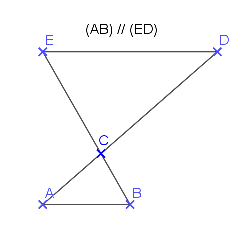
\includegraphics[scale=1]{qcm2.eps}
 \end{center} 


\exo{5}


\begin{center}
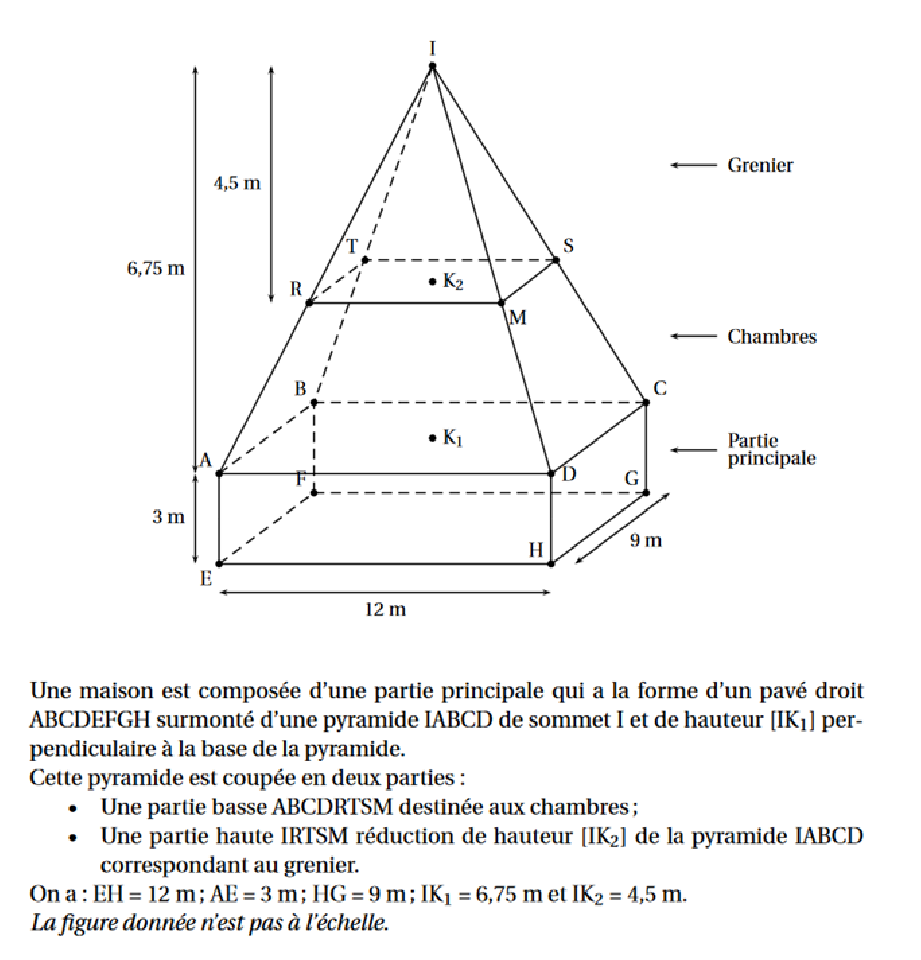
\includegraphics[scale=0.9]{exo1.eps} 
\end{center}


\newpage

\begin{center}
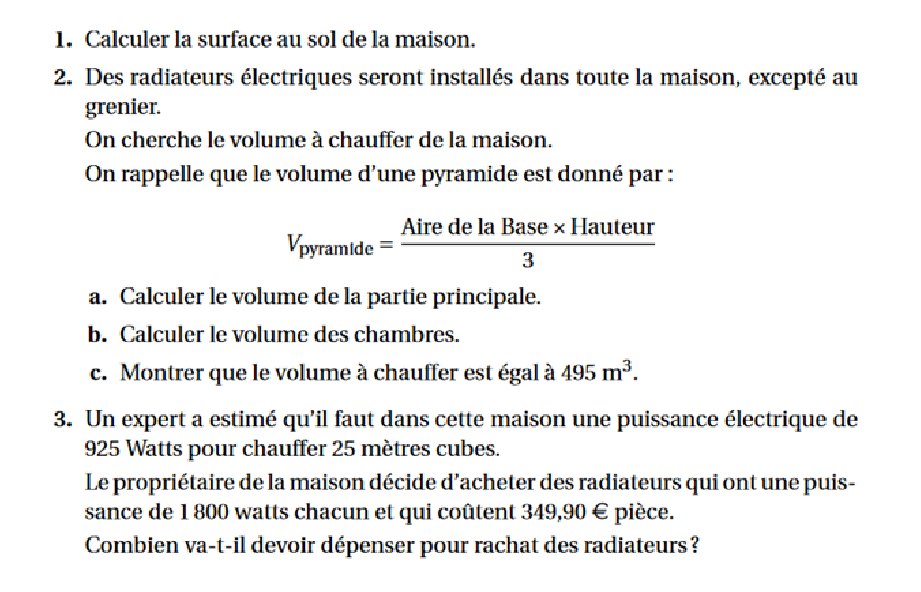
\includegraphics[scale=0.9]{exo2.eps} 
\end{center}


\exo{7}


\begin{center}
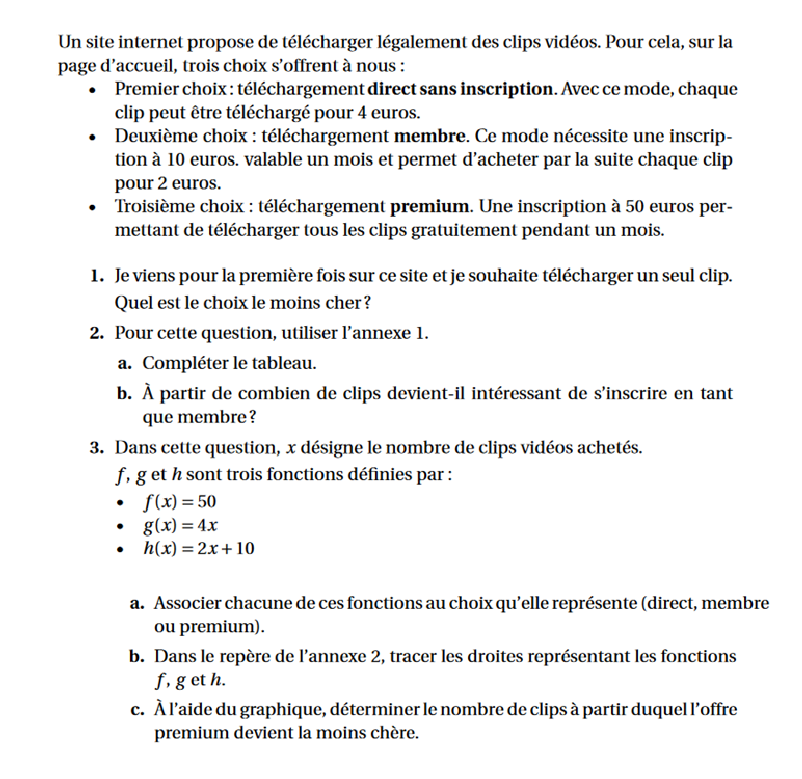
\includegraphics[scale=1.1]{exo3.eps} 
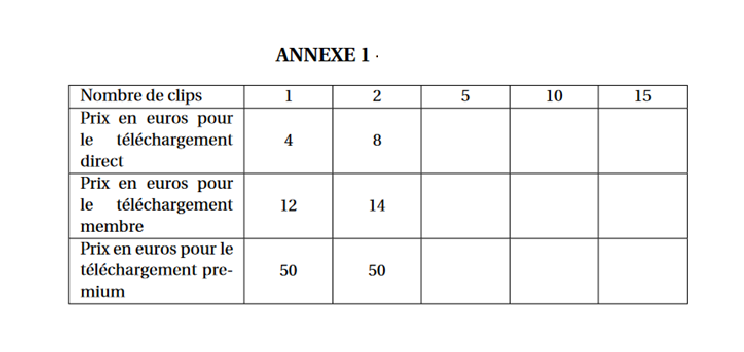
\includegraphics[scale=0.9]{exo4.eps} 
\end{center}

\newpage

\begin{center}
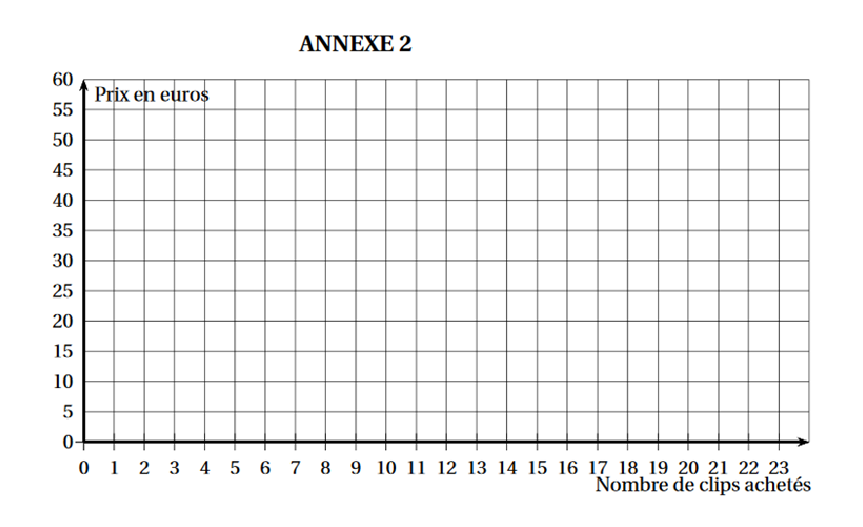
\includegraphics[scale=1]{exo5.eps} 
\end{center}


\exo{6.75}

\bmul{4}

$f(x) = 2x$\\

$p(x) = (3x-1)^{2} -3x^{2}$

\columnbreak

$g(x) = x^{2}$\\

$k(x) = -x$

\columnbreak

$h(x) = \dfrac{1}{x}$\\

$d(x) = \dfrac{x}{3} + 10 $

\columnbreak

$i(x) = 4x-3$\\

$j(x) = 321$



\emul


\q Parmi les fonctions définies ci-dessus, indiquer celles qui sont affines (en précisant celles qui sont linéaires ou constantes ainsi que leur coefficient.)\\

\q Calculer l'image 9 par la fonction $d$.\\

\q Calculer l'image de -2 par la fonction $k$.\\

\q Calculer l'antécédent de 25 par la fonction $i$.\\

\q Calculer l'antécédent de 0 par la fonction $p$.\\





\end{document}
